% Configuration

\documentclass[a4paper]{article}

\linespread{1.1}

\usepackage[utf8]{inputenc} 
\usepackage[T1]{fontenc}
\usepackage[francais]{babel}
\usepackage{amsmath}
\usepackage{amsfonts}
\usepackage{graphicx}
\usepackage{lmodern}
\usepackage{microtype}
\usepackage{hyperref}
\usepackage[margin=1.8cm]{geometry}
\usepackage{pgf,tikz}
\usepackage{mathrsfs}
\usetikzlibrary{arrows}


% Structure

\newcounter{c}
\newcounter{d}
\newcounter{r}
\newcounter{e}

\newcommand{\defi}{\subparagraph{D\'efinition \arabic{c}.\arabic{d} :}\stepcounter{d}}
\newcommand{\prop}{\subparagraph{Proposition \arabic{c}.\arabic{r} :}\stepcounter{r}}
\newcommand{\thm}{\subparagraph{Th\'eor\`eme \arabic{c}.\arabic{r} :}\stepcounter{r}}
\newcommand{\demo}{\subparagraph{D\'emonstration}}
\newcommand{\cor}{\subparagraph{Corollaire \arabic{c}.\arabic{r} :}\stepcounter{r}}
\newcommand{\lem}{\subparagraph{Lemme \arabic{c}.\arabic{r} :}\stepcounter{r}}
\newcommand{\rem}{\subparagraph{Remarque :}}
\newcommand{\chapitre}[1]{\stepcounter{c}\setcounter{e}{0}\setcounter{d}{0}\setcounter{r}{0}\noindent\textbf{\Large\arabic{c}. #1}\\}
\newcommand{\eq}[1]{\stepcounter{e}\begin{equation}#1\tag{\arabic{c}.\arabic{e}}\end{equation}}

% Notations

\newcommand{\Q}{\mathbb{Q}}
\newcommand{\Z}{\mathbb{Z}}
\newcommand{\N}{\mathbb{N}}
\newcommand{\R}{\mathbb{R}}
\newcommand{\C}{\mathbb{C}}
\newcommand{\E}[1]{\mathbb E\left(#1\right)}
\newcommand{\sph}{\mathbb{S}}
\newcommand{\p}{{\cal{P}}}
\newcommand{\fsp}{{\cal{F}}}
\newcommand*{\qed}{\hfill\ensuremath{\square}}
\newcommand{\x}{\mathbf x}
\newcommand{\y}{\mathbf y}
\newcommand{\e}{\mathbf e}
\newcommand{\scal}[2]{\langle#1,#2\rangle}
\newcommand{\trans}{^\text{T}\!}

\newcommand{\nor}[2]{{\cal N}(#1,#2)}
\newcommand{\mat}[2]{{\cal M}_{#1\times#2}(\R)}

\newcommand{\X}{\mathbf X}

\date{}
\author{Philippe Ricka}
\title{}

\newcommand{\saut}{\vspace{0.5em}}

\begin{document}

%\maketitle

\chapitre{Filtre de Kalman discret (KF)}

On considère un système dynamique stochastique linéaire

\eq{\left\{\begin{array}{l}x_{k+1}=A_kx_k+w_k\\y_k=H_kx_k+v_k\end{array}\right.}

Où
\begin{itemize}
\item $\x_k\in\R^n$ désigne l'état du système
\item $A_k\in\mat nn$ désigne la matrice de transition relative à la dynamique réelle
\item $\y_k\in\R^m$ désigne les mesures relatives à l'état réel $\x$
\item $H_k\in\mat mn$ désigne la matrice de mesure
\item $v_k\in\R^m$ désigne l'erreur d'obervation, qu'on suppose $\nor 0{R_k}$
\item $w_k\in\R^n$ désigne la perturbation du système, qu'on suppose $\nor 0{Q_k}$
\end{itemize}
On suppose de plus que $v_k$ et $w_k$ sont indépendantes.


On mettra en exposant un $f$ (\emph{forecast}) pour les prévisions et un $a$ (\emph{analysis}) pour les analyses.

\saut

On postule l'absence d'erreur du modèle pour la prédiction à partir d'une analyse.

$$\x^f_{k+1}=A_k\x^a_k$$

Une estimation de l'état du système à un instant $t_k$ (analyse) est supposément une combinaison linéaire de la prédiction actuelle et des mesures actuelles.

$$\x^a_k=\tilde L_k\x^f_k+\tilde K_k\y_k\text{ où $\tilde L_k\in\mat nn$ et $\tilde K_k\in\mat nm$ sont des matrices à préciser}$$

On définit formellement les erreurs de prédiction et d'analyse.

$$\begin{array}{lr}\e^f_k=\x^f_k-\x_k&\e^a_k=\x^a_k-\x_k\end{array}$$

où $\x_k$ désigne l'état réel du système.

\prop Si $\tilde L_k=I-\tilde K_kH_k$ et si $\E{\e^f_k}=0$, alors $\E{\e^a_k}=0$.
\demo $$\begin{array}{rl}
\E{\e^a_k}=&\E{\x^a_k}-\x_k\\
=&\E{\tilde L_k\x^f_k+\tilde K_k\y_k}-\x_k\\
=&\E{(I-\tilde K_kH_k)\x^f_k+\tilde K_k\y_k}-\x_k\\
=&\E{\x^f_k-\tilde K_kH_k\x^f_k+\tilde K_k(H_k\x_k+v_k)}-\x_k\\
=&\E{(I-\tilde K_kH_k)\e^f_k}\\
=&0
\end{array}$$\qed

\defi On appelle $\tilde K_k$ la \emph{matrice de gain}. Elle décrit les poids attribués aux observations $\y_k$ et aux mesures $H_k\x^f_k$.

On définit les covariances des erreurs de prévision et d'analyse.

\eq{\begin{array}{lr}P^f_k=\E{\e^f_k\cdot\trans\e^{f}_k}&P^a_k=\E{\e^a_k\cdot^\text{T}\e^{a}_k}\end{array}}

\prop Sous les hypothèses de la proposition précédente, on a :

\eq{\begin{array}{rl}
P^a_k=&(I-\tilde K_kH_k)\cdot P^f_k\cdot\trans(I-\tilde K_kH_k)+\tilde K_k\cdot R_k\cdot\trans\tilde K_k\\
&\\
P^f_k=&A_k\cdot P^a_k\cdot\trans A_k-Q_k
\end{array}}
\demo On pose $Cov(\x)=\E{\x\cdot\trans\x}$.
$$\begin{array}{rl}
P^a_k=&\E{\e^a_k\cdot\trans\e^a_k}=Cov(\e^a_k)\\
=&Cov\left(\tilde L_k\x^f_k+\tilde K_k\y_k-\x_k\right)\\
=&Cov\left((I-\tilde K_kH_k)\x^f_k+\tilde K_k\y_k-\x_k\right)\\
=&Cov\left((I-\tilde K_kH_k)\x^f_k+\tilde K_k(H_k\x_k+v_k)-\x_k\right)\\
=&(I-\tilde K_kH_k)\cdot Cov\left(\x^f_k-\x_k\right)\cdot\trans(I-\tilde K_kH_k)+Cov\left(\tilde K_kv_k\right)\\
=&(I-\tilde K_kH_k)\cdot P_k^f\cdot\trans(I-\tilde K_kH_k)+\tilde K_k\cdot R_k\cdot\trans\tilde K_k\\
&\\
P^f_{k+1}=&Cov\left(\e_{k+1}^f\right)\\
=&Cov\left(\x^f_{k+1}-\x_{k+1}\right)\\
=&Cov\left(A_k\x^a_k-A_k\x_k-w_k\right)\\
=&A_k\cdot Cov(e_k^a)\cdot\trans A_k-Cov\left(w_k\right)\\
=&A_k\cdot P_k^a\cdot\trans A_k-Q_k
\end{array}$$\qed

\rem Dans un modèle parfait, on aurait $Q_k=0$.

\saut

On contruit maintenant ${\mathcal I}_k^a$, un estimateur de la fiabilité des analyses, en mesurant l'écart entre l'analyse et le véritable état. Soit $B_k\in\mat nn$ déterministe diagonale définie positive : la matrice d'échelle. On pose :

\eq{{\cal I}_k^a=\E{\trans\e^a_k\cdot B_k\cdot\e^a_k}=\E{\sum_{i=1}^n(\e^a_k)_im_{ii}(\e^a_k)_i}=\text{Tr}(B_kP^a_k)}

On souhaite minimiser ${\cal I}_k^a$. Cela revient à minimiser $P^a_k$. On va différencier l'application $\varphi:\mat nn\to\R,\tilde K_k\mapsto P^a_k$.
$$\begin{array}{rl}\varphi(\tilde K_k+h)=&(I-(\tilde K_k+h)H_k)\cdot P_k^f\cdot\trans(I-(\tilde K_k+h)H_k)+(\tilde K_k+h)\cdot R_k\cdot\trans(\tilde K_k+h)\\
=&P^f_k-\tilde K_k\cdot H_k\cdot P^f_k-P_k^f\cdot\trans H_k\cdot\trans\tilde K_k+\tilde K_k\cdot H_k\cdot P^f_k\cdot\trans H_k\trans\tilde K_k+\tilde K_k\cdot R_k\cdot\trans\tilde K_k\\
&-h\cdot H_k\cdot P^f_k-P^f_k\cdot\trans H_k\cdot\trans h+h\cdot H_k\cdot P^f_k\cdot\trans H_k\cdot\trans\tilde K_k\\
&+\tilde K_k\cdot H_k\cdot P^f_k\cdot\trans H_k\cdot\trans h+h\cdot R_k\cdot\trans\tilde K_k+\tilde K_k\cdot R_k\cdot\trans h\\
&+h\cdot H_k\cdot P^f_k\cdot\trans H_k\cdot\trans h+h\cdot R_k\cdot\trans h
\end{array}$$

d'où

$$d(\varphi)(\tilde K_k)(h)=-h\cdot (H_k\cdot P^f_k\cdot (I-\trans H_k\cdot \trans\tilde K_k)-R_k\cdot \trans\tilde K_k)-((I-\tilde K_k\cdot  H_k)P^f_k\cdot \trans H_k-\tilde K_k\cdot R_k)\cdot \trans h$$

On cherche $\tilde K_k$ optimale, c'est à dire telle que $d(\varphi)(\tilde K_k)=0$. C'est le cas lorsque :

$$H_k\cdot\trans P^f_k\cdot(I-\trans H_k\cdot\trans\tilde K_k)-\trans R_k\cdot\trans\tilde K_k=0$$

donc lorsque :

\eq{\tilde K_k=P^f_k\cdot\trans H_k\cdot\left(H_k\cdot P^f_k\cdot\trans H_k+R_k\right)^{-1}:=K_k.}

Cette matrice $K_k\in\mat nm$ est appelée le \emph{gain de Kalman}. En l'injectant dans l'expression de $P^a_k$, on trouve

$$\begin{array}{rl}
P^a_k=&(I-K_k\cdot H_k)\cdot P^f_k\cdot\trans(I-K_k\cdot H_k)+K_k\cdot R_k\cdot\trans K_k\\
=&P^f_k-P^f_k\cdot\trans H_k\cdot(H_k\cdot P^f_k\cdot\trans H_k+R_k)^{-1}\cdot H_k\cdot P^f_k\\
&-P^f_k\cdot\trans H_k\cdot(H_k\cdot\trans P^f_k\cdot\trans H_k+\trans R_k)^{-1}\cdot H_k\cdot\trans P^f_k\\
&+P^f_k\cdot\trans H_k\cdot(H_k\cdot\trans P^f_k\cdot\trans H_k+\trans R_k)^{-1}\cdot H_k\cdot\trans P^f_k\\
=&P^f_k\cdot(I-\trans H_k\cdot\trans K_k)\\
=&(I-H_k\cdot K_k)\cdot P^f_k
\end{array}$$

La dernière égalité ayant lieu grâce au caractère symétrique de $P^f_k$.

\newpage
On aboutit finalement à la relation :

\eq{\x^a_k=\x^f_k+K_k(\y_k-H_k\x^f_k).}

La procédure s'itère dans le temps suivant les étapes :

\saut

\begin{tabular}{p{3cm}|l}
Analyse &$K_k = P^f_k\cdot H_k\cdot(H_k\cdot P^f_k\cdot \trans H_k + R_k)^{-1}$\\
&$\x^a_k = \x^f_k + K_k\cdot(\y_k - H_k\cdot\x^f_k)$\\
&$P^a_k = (I-K_k\cdot H_k)\cdot P^f_k$\\
\end{tabular}

\saut

\begin{tabular}{p{3cm}|l}
Prédiction &$\x^f_{k+1} = A_k\cdot \x^a_k$\\
&$P^f_{k+1} = A_k\cdot P^a_k\cdot\trans A_k +Q_k$
\end{tabular}


\begin{figure}[!h]
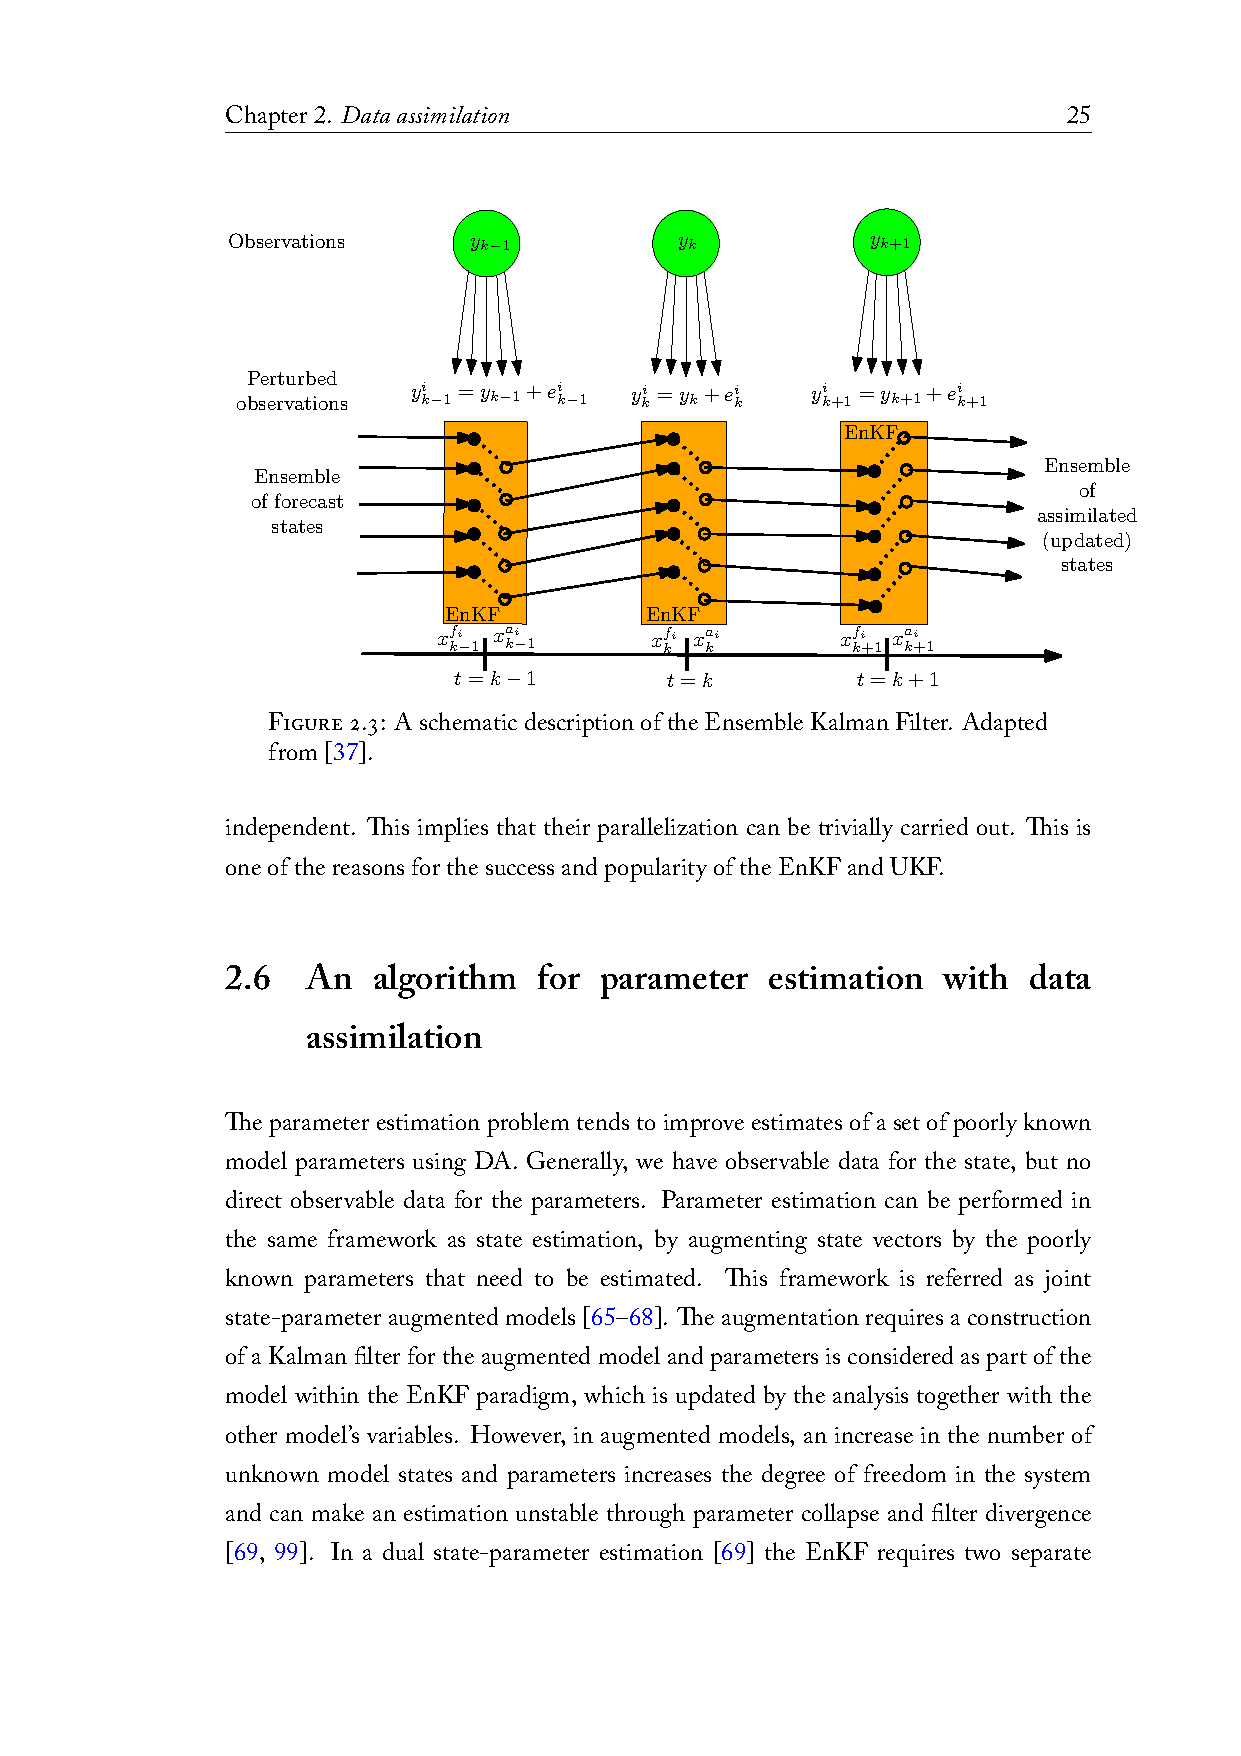
\includegraphics[width=\textwidth,trim = 3.5cm 18.1cm 3cm 3.5cm, clip]{kfchart.pdf}
\caption{Fonctionnement général du KF}
\end{figure}

\newpage
\chapitre{Exemple : chute d'un mobile}

On considère la chute d'un mobile soumis à une accélération de la pesanteur $g$ au cours d'un intervalle de temps $[0,T]$ discrétisé avec un pas $dt$. On note sa position, sa vitesse et son accélération au temps $k.dt$ respectivement $x_k$, $x'_k$ et $x''_k$. Le vecteur d'état du système à un instant $k.dt$ est :

$$\x_k=\left(\begin{matrix}x_k\\x'_k\\x''_k\end{matrix}\right).$$

La physique nous renseigne sur la matrice de transition $A$ d'un instant au suivant :

$$A=\left(\begin{matrix}1&dt&dt^2\\0&1&dt\\0&0&1\end{matrix}\right)$$

de façon à ce que la relation de récurrence suivante ait lieu :

$$\x_{k+1}=A\cdot\x_k+\mathbf w_k$$

où $\mathbf w_k\sim\mathcal{N}(0,Q)$ pour une matrice de covariance $Q$ fixée. En supposant que les bruits affectant la position, la vitesse et l'accélération sont indépendants, on trouve :

$$Q=\left(\begin{matrix}(w_k)^2&0&0\\0&(w_k')^2&0\\0&0&(w_k'')^2\end{matrix}\right).$$

On relève à chaque instant l'état du système en commettant une erreur $\mathbf v_k$ :

$$\y_k=H\cdot\x_k+\mathbf v_k=\x_k+\mathbf v_k$$

en prenant $H=I_3$, où $\mathbf v_k\sim\mathcal N(0,R)$ pour une matrice de covariance diagonale fixée $R$ (on suppose les erreurs de mesure indépendantes).

\saut

En considérant le pas de temps $dt$ suffisamment petit, il est raisonnable d'initialiser \verb Pf= $P^f_1=R$.

Les matrices impliquées dans nos calculs ont des expressions relativement simples grâce à l'hypothèse $H=I_3$, qui revient à supposer que l'on mesure directement les grandeurs qui nous intéressent.

\newpage
\begin{verbatim}

génération des états réels x_k bruités par w_k de covariance Q
génération des mesures y_k bruitées par v_k de covariance R

Pf = R ;
xf(1) = y(1);

pour k de 2 à T/dt
    K = Pf * inv(Pf + R);
    xa = xf(:,i-1) + K * (y(:,i) - xf(:,i-1));
    Pa = (I - K) * Pf;
  
    xf(:,i) = A * xa;
    Pf = A * Pa * A' + Q;
fin

\end{verbatim}


La figure 1 illustre les résultats obtenus pour la position et la vitesse d'un mobile dans le cas où :
\begin{itemize}
\item $g=-9.81 m.s^{-2}$,
\item $dt=0.2 s$,
\item $T=5 s$,
\item $\x_1=\trans\left(\begin{matrix}0&0&0\end{matrix}\right)$,
\item $w_k=1$, $w_k'=0.5$, $w_k''=0.25$,
\item $v_k=5$, $v_k'=5$, $v_k''=10$.
\end{itemize}




\begin{figure}[!h]
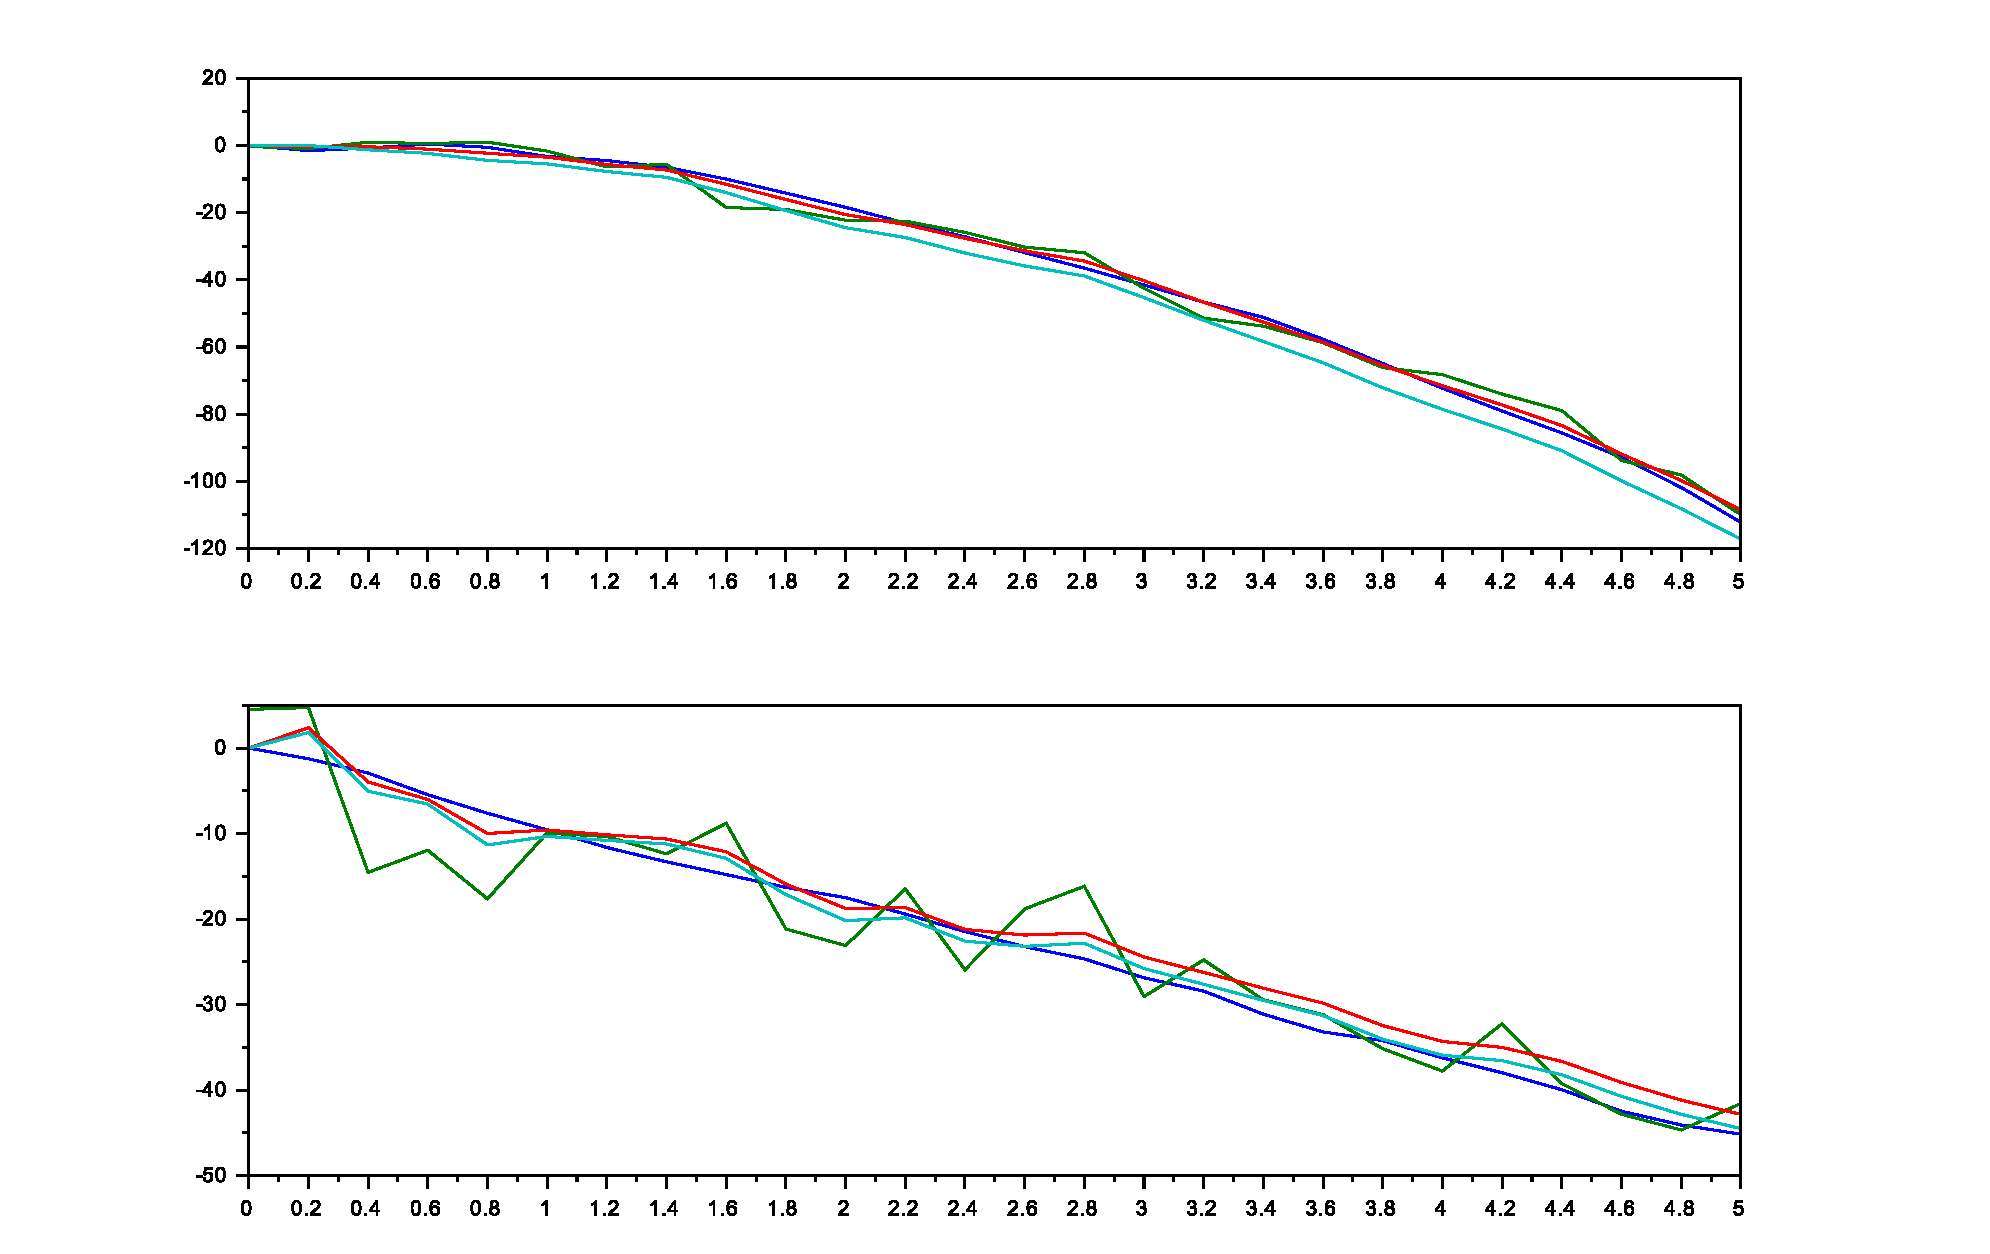
\includegraphics[width=\textwidth]{KalmanMobile.pdf}
\caption{En bleu : $\x$. ; en vert : $\y$ ; en rouge : $\x^a$ ; en cyan : $\x^f$.}
\end{figure}


\newpage
\chapitre{Ensemble Kalman Filter (EnKF) - explicit dynamics}

Ce filtre fonctionne sur le meme principe que le KF, à ceci près qu'on évalue $P^f_k$ à partir d'un ensemble $\{\x^{fi}_k|i=1,...,q_{ens}\}$ où $q_{ens}>1$ est un entier. Dans le cas où la dynamique du système est décrite par une fonction linéaire ou par une fonction très régulière, on préfèrera le KF appliqué à cette fonction ou à la fonction linéarisée pour des raisons de coût. En revanche, l'EnKF dévoile ses performances dans le cas des processus non-linéaires. En toute généralité :

\eq{\left\{\begin{array}{l}\x_{k+1} = f(\x_k,\mathbf u_k)+\mathbf w_k\\\y_k=h(\x_k)+\mathbf v_k\end{array}\right.}

où les notations employées sont les mêmes que précédemment, et $f$ désigne la fonction décrivant la dynamique du système et $\mathbf u_k$ est un paramètre du système.



Au premier pas, on se munit d'un ensemble d'estimations initiales $\X_1 = \{\x^{fi}_1|i=1,...,q_{ens}\}$, et on suppose à chaque pas qu'on dispose d'une telle famille $\X_k$. On définit la prédiction moyenne :

\eq{\overline{\x_k^f}=\frac1{q_{ens}}\sum_{i=1}^{q_{ens}}\x_k^{fi}.}

La matrice de covariance de l'erreur de prédiction est alors :

\eq{P^f_k=\frac1{q_{ens}-1}\sum_{i=1}^{q_{ens}}(\x_k^{fi}-\overline{\x_k^f})\cdot\trans(\x_k^{fi}-\overline{\x_k^f}).}


On bruite $q_{ens}$ fois la mesure de façon à produire une famille $\{\y_k^i=\y_k+\mathbf e_k^i|i=1,...,q_{ens}\}$ où chaque $\mathbf e_k^i$ est gaussien de taille $m$ et de faible variance.


Pour calculer le gain de Kalman, il est nécessaire de construire la matrice $R_k$. Par indépendance des bruits, elle doit être diagonale. On trouve dans la littérature l'approximation :

\eq{R_k \simeq \text{diag}\left(\frac1{q_{ens}-1}E\cdot\trans E\right)}

où $E=(\mathbf e_k^1,...,\mathbf e_k^{q_{ens}})\in\mat m{q_{ens}}.$

Le gain de Kalman s'exprime de la même façon que dans le cas précédent ; toutefois, $H_k$ désigne l'approximation linéaire de $h$ au voisinage de $\x_k$, ce qui peut être délicat à calculer. D'après Houtekamer et Mitchell si $\overline{h(\x_k^f)}=h(\overline{\x_k^f})$ et si $\|\x_k^{fi}-\overline{\x_k^f}\|$ est assez petit pour tout $i$, alors les approximations suivantes sont raisonnables :

\eq{P^f_{\x\y_k}=P^f_k\cdot\trans H_k\simeq\frac1{q_{ens}-1}\sum_{i=1}^{q_{ens}}(\x_k^{fi}-\overline{\x_k^f})\cdot\trans(h(\x_k^{fi})-h(\overline{\x_k^f}))}

\eq{P^f_{\y\y_k}=H\cdot P^f_k\cdot\trans H+R_k\simeq\frac1{q_{ens}-1}\sum_{i=1}^{q_{ens}}(h(\x_k^{fi})-\overline{h(\x_k^f)})\cdot\trans(h(\x_k^{fi})-\overline{h(\x_k^f)})+R_k.}



Il suffit alors de remarquer que :

\eq{K_k = P^f_{xy_k}\cdot\left(P^f_{yy_k}\right)^{-1}.}


En somme, on applique l'algorithme suivant :

\begin{verbatim}
pour k de 2 à T/dt
    pour i de 1 à qens
        xf(i) = f(xa(i),uk) + w(i);
    fin
    Pxy = formule (3.5);
    Pyy = formule (3.6);
    K = Pxy*inv(Pyy);
    pour i de 1 à qens
        y(i) = yk + e(i);
        xa(i) = xf(i) + K*(y(i) -  h(xf(i)))
    fin
fin
\end{verbatim}


\begin{figure}
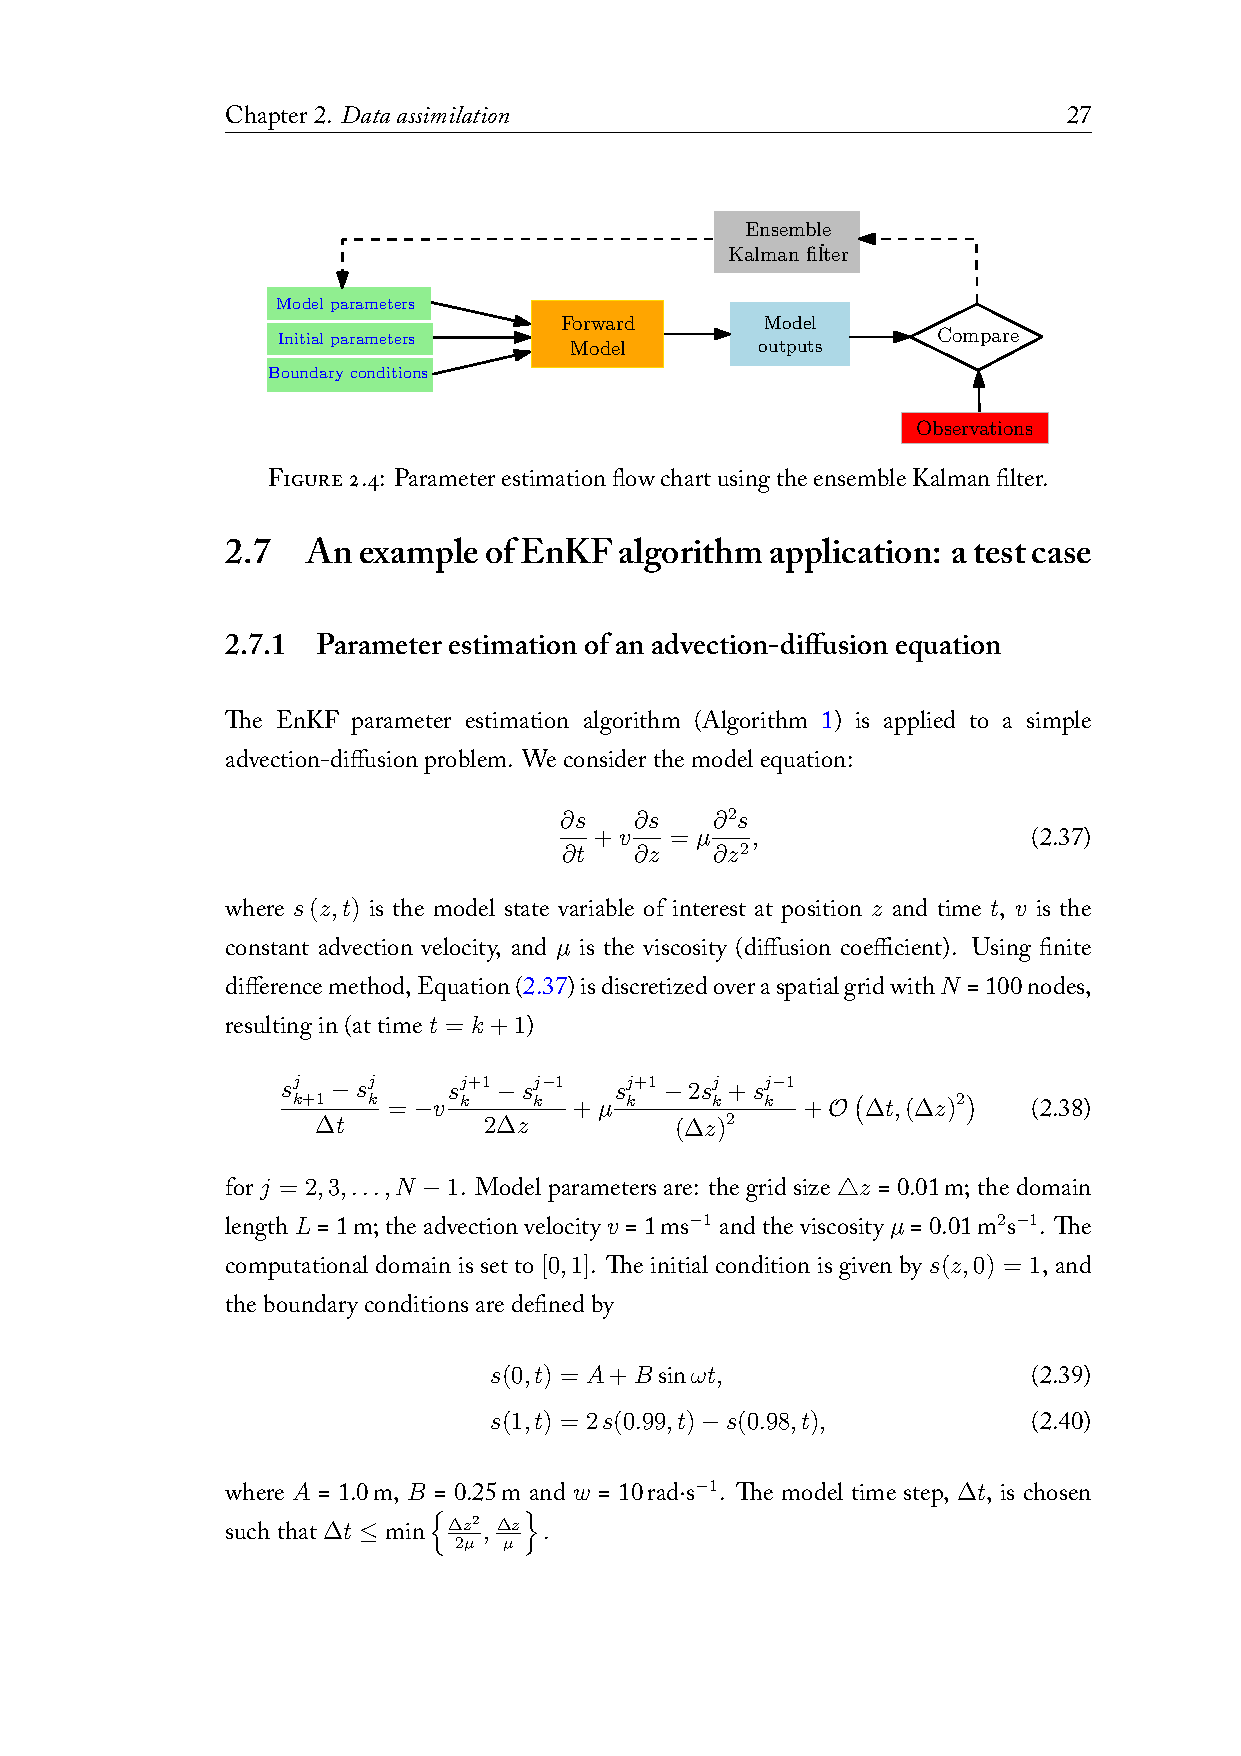
\includegraphics[width=\textwidth,trim = 3.85cm 22.1cm 1.8cm 3.5cm, clip]{enkfchart.pdf}
\caption{Fonctionnement du EnKF}
\end{figure}





\chapitre{Ensemble Kalman Filters : implicit dynamics}

Il arrive souvent que l'utilisateur n'ait pas accès directement à la fonction $f$ relative à la dynamique du système. Dans ce cas, on peut se contenter d'admettre que $x^f$ suit une marche aléatoire :

\eq{x^f_{k+1}=x^f_k+\delta_k}

où $\delta_k\sim\nor0{D_k}$. En reprenant l'exemple précédent, on condsidère que la marche aléatoire concerne indépendamment chaque composante de $\x$. La matrice $D_k$ est alors diagonale. Dans le but d'approcher la dynamique réelle, choisissons :

$$D_k(1,1)=(x_k-x_{k-1})^2=(x'_0dt+g(2k-1)dt^2)^2$$
$$D_k(2,2)=(x'_k-x'_{k-1})^2=(gdt)^2$$

La matrice $D_k$ devant être définie positive, on choisit un $\varepsilon>0$ très petit et on pose :

$$D_k(3,3)=\varepsilon.$$

Dans l'exemple, nous avons arbitrairement pris $\varepsilon=dt$.


\begin{figure}[!h]
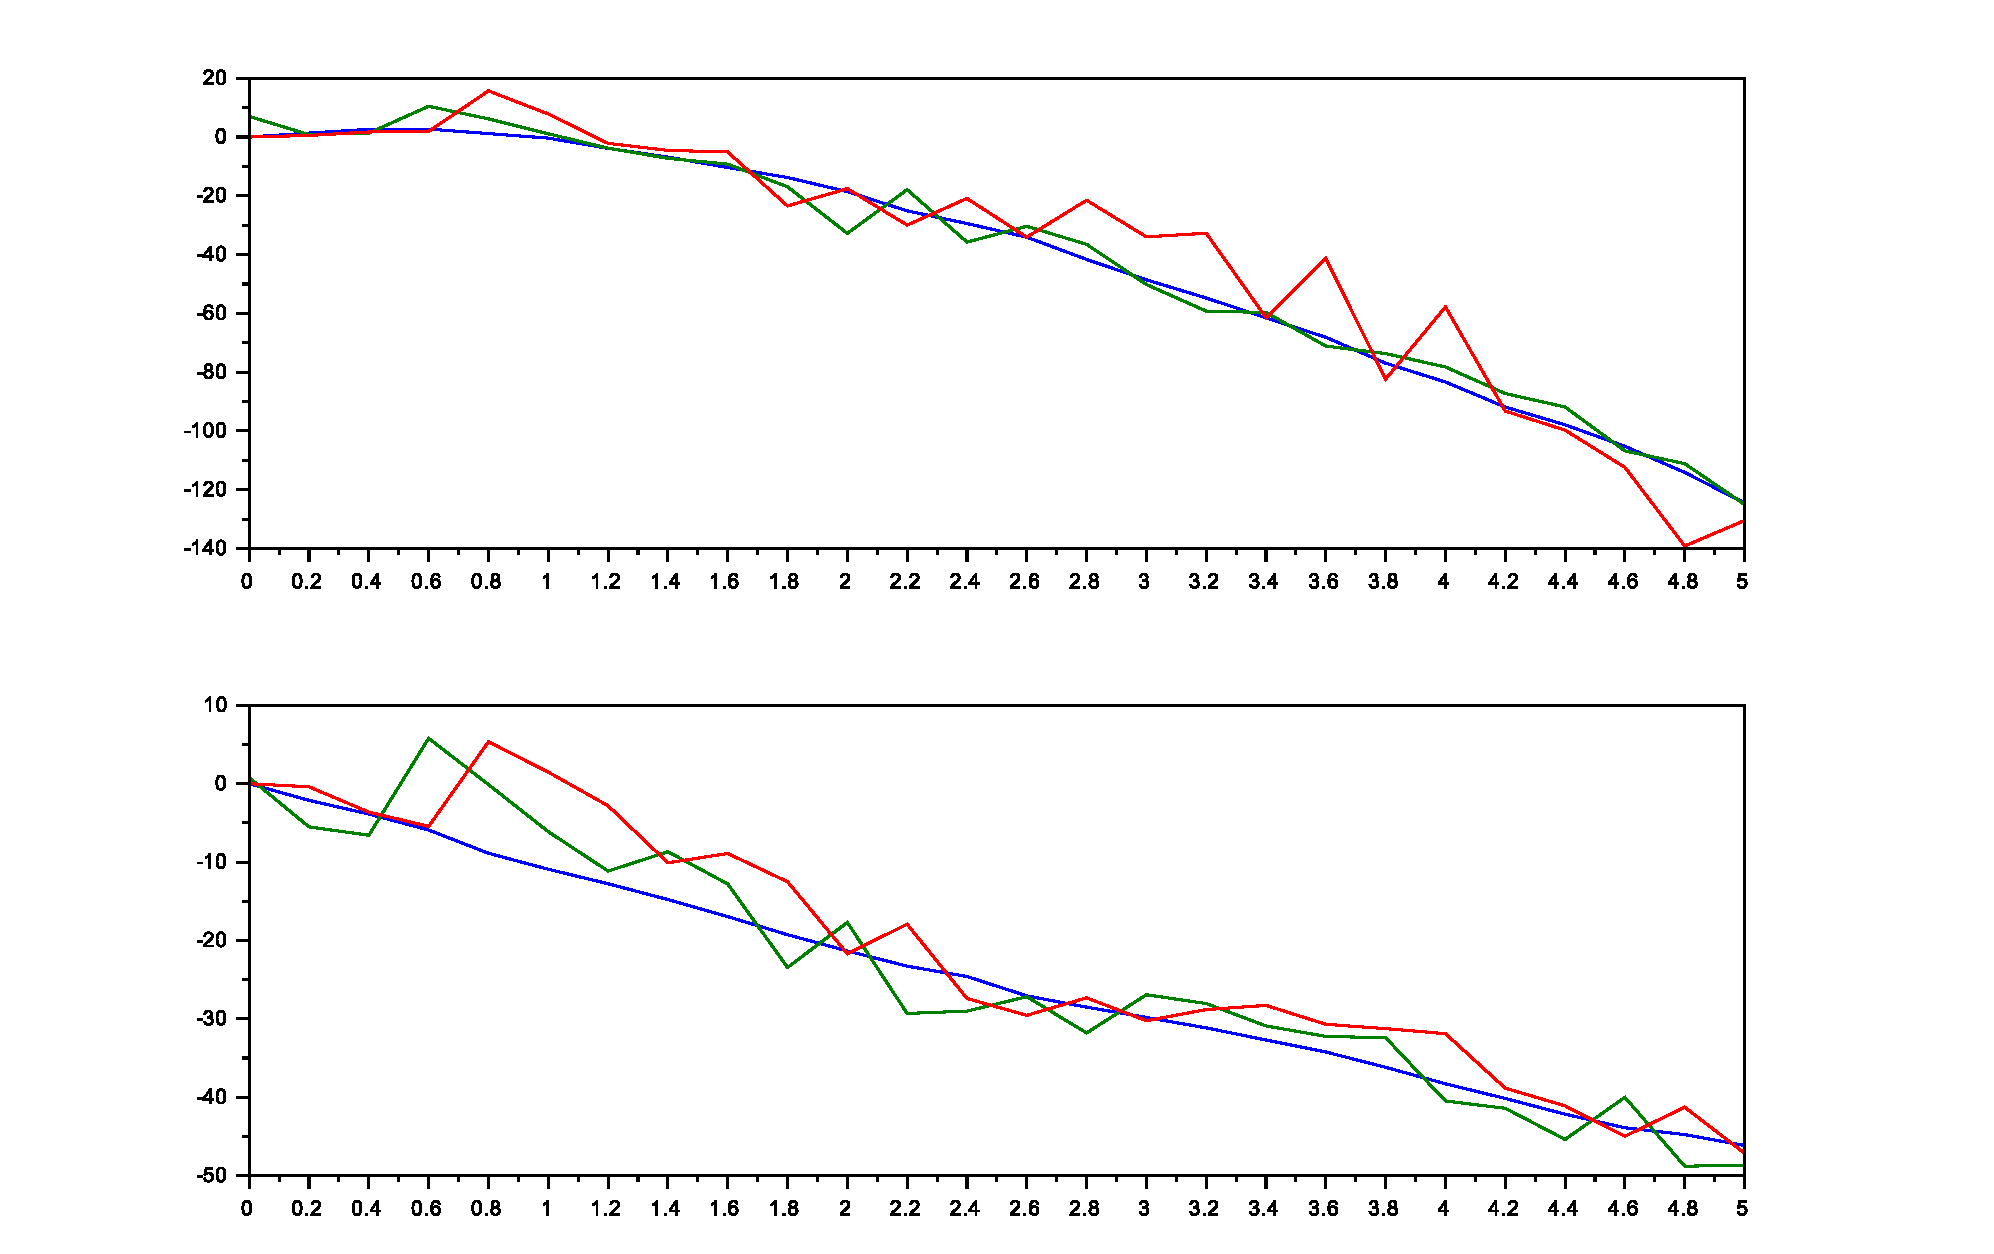
\includegraphics[width=\textwidth]{ENKalmanMobile.pdf}
\caption{En bleu : $\x$ ; en vert : $\y$ ; en rouge : $\overline{\x^f}$.}
\end{figure}

L'algorithme devient :

\begin{verbatim}
pour k de 2 à T/dt
    Dk = diag( (y1(2)*dt + g*(2*k-1)*dt)^2 , (g*dt)^2 , dt);
    pour i de 1 à qens
        xf(i) = xa(i) + delta;
        yk(i) = yk + e;
    fin
    Pxy = formule (3.5);
    R = formule (3.4);
    Pyy = formule (3.6);
    K = Pxy*inv(Pyy);
    pour i de 1 à qens
        xa(i) = xf(i) + K*(y(i) - h(xf(i)));
    fin
fin

\end{verbatim}


On voit que la fonction dynamique $f$ n'intervient à aucun moment. La prédiction est évidemment moins précise que dans le cas discret, mais cette méthode permet de produire une prédiction à propos d'un système dont on ne connait \emph{a priori} pas la dynamique. Sur le même exemple que précédemment, on obtient les résultats représentés dans la figure 2.


Ce type de filtre de Kalman permet en particulier d'estimer les paramètres d'un système. Dans sa thèse, R. Lal obtient d'excellentes estimations de la viscosité, de la vitesse d'advection et des conditions initiales dans le cadre de l'équation d'advection-diffusion avec $q_ens = 4$, $T=100$, $dt=0,15$, à partir d'une simulation \emph{in silico}.


\newpage
\chapitre{Additional examples}

We consider a lumped 0D RCR model for a tubular elastic blood vessel : a resistor $R_1$ at the flow input $q(t)$ connected to a grounded (output) resistor $R_2$ and a grounded capacitor $C$. The total pressure (input-to-ground voltage) is denoted by $p$, and $\pi$ the nodal pressure (node-to-ground voltage).


\begin{center}
\begin{tikzpicture}
\draw (-1.7,0)--(-1.3,0);
\draw (1.3,0)--(1.7,0);
\draw (0,-1)--(0,-1.4);
\draw (-0.7,0)--(0.7,0);
\draw (0,0)--(0,-0.8);

% resistors
\draw (-1.3,0)--(-1.2,0.2)--(-1.1,-0.2)--(-1,0.2)--(-0.9,-0.2)--(-0.8,0.2)--(-0.7,0);
\draw (1.3,0)--(1.2,0.2)--(1.1,-0.2)--(1,0.2)--(0.9,-0.2)--(0.8,0.2)--(0.7,0);

% capacitor
\draw (-0.25,-0.8)--(0.25,-0.8);
\draw (-0.25,-1)--(0.25,-1);

% ground
\draw (-0.25,-1.4)--(0.25,-1.4);
\draw (-0.18,-1.45)--(0.18,-1.45);
\draw (-0.11,-1.5)--(0.11,-1.5);
\draw (-0.06,-1.55)--(0.06,-1.55);

\draw (1.7,0.25)--(1.7,-0.25);
\draw (1.75,0.18)--(1.75,-0.18);
\draw (1.8,0.11)--(1.8,-0.11);
\draw (1.85,0.06)--(1.85,-0.06);

% annotations
\draw (0,0) node [above] {$\pi$};

\draw (-1,0.3) node [above] {$R_1$};
\draw (1,0.3) node [above] {$R_2$};
\draw (0.3,-0.85) node [right] {$C$};

\draw[->] (-2.15,0)--(-1.75,0);
\draw (-2,0) node [above] {$p$};
\draw (-2,0) node [below] {$q$};

\end{tikzpicture}


~


$RCR~network$
\end{center}

The relation between $p$ and $q$ writes :

$$C\frac d{dt}p+\frac p{R_2}=CR_1\frac d{dt}q+\left(1+\frac{R_1}{R_2}\right)q$$

Taking Gerbeau's flow input (p26 of his beamer), we first tried to recover pressure from noised measurements, then to recover the prescribed flow using pressure measurements only, the parameters $R_1=1300\Omega,R_2=16000\Omega,C=0.000025F$ being known. The following graphs sum up the results in the cases $q_{ens}=10$ and $q_{ens}=1000$ : the top graph illustrates pressure estimation (real $p$ in blue, measurement in red, estimation in yellow) and the bottom graph illustrates flow estimation (real $q$ in blue, estimation in red).

\begin{center}
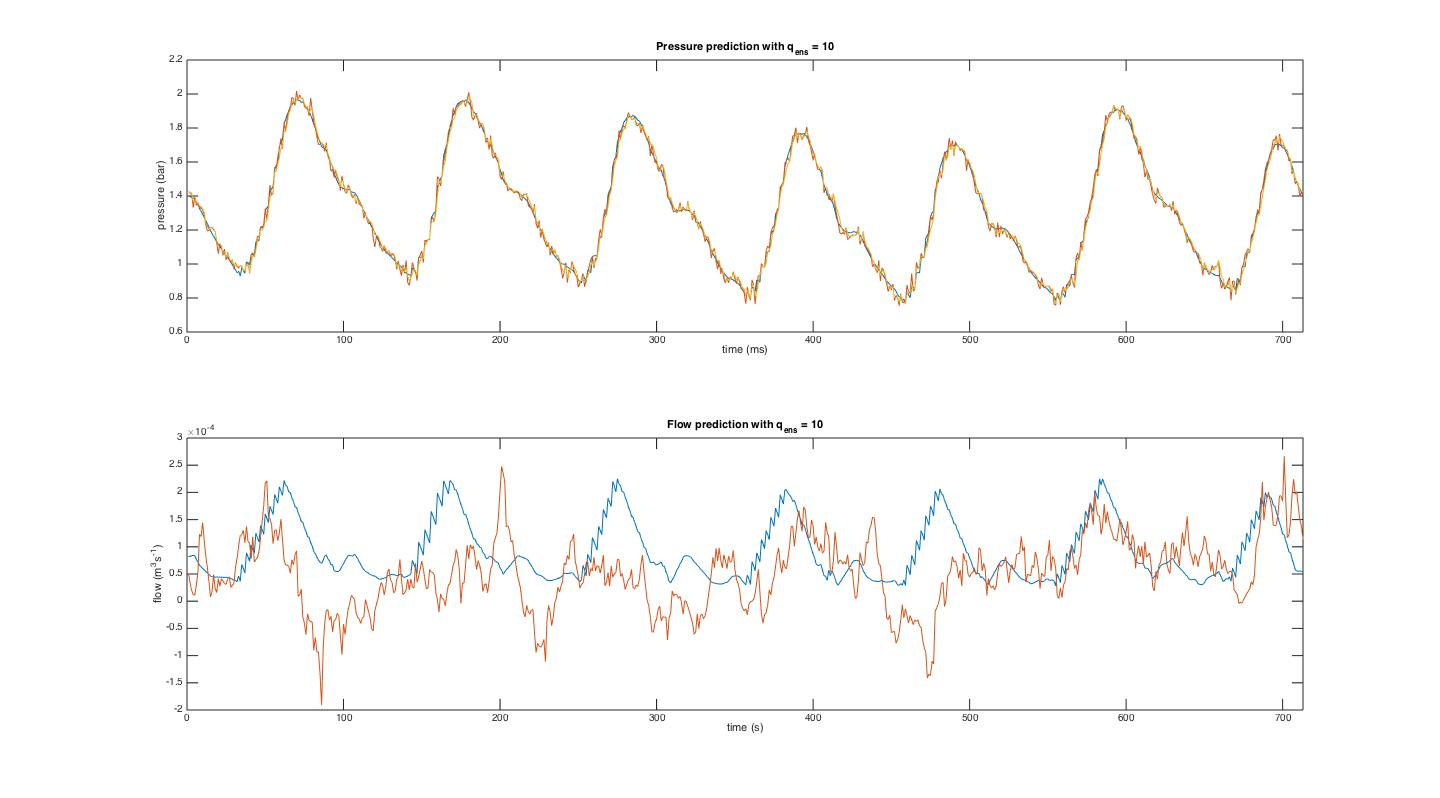
\includegraphics[width=\textwidth]{KFex1}
\end{center}

If $p$ is the real pressure, $y$ its measurement and $x$ its estimation based on $y$, we get a ratio (sum of $(p-y)^2$)/(sum of $(p-x)^2$) = $1.2242$ and a mean square difference between $q$ and its estimation of $1.136810^{-8}$.

\begin{center}
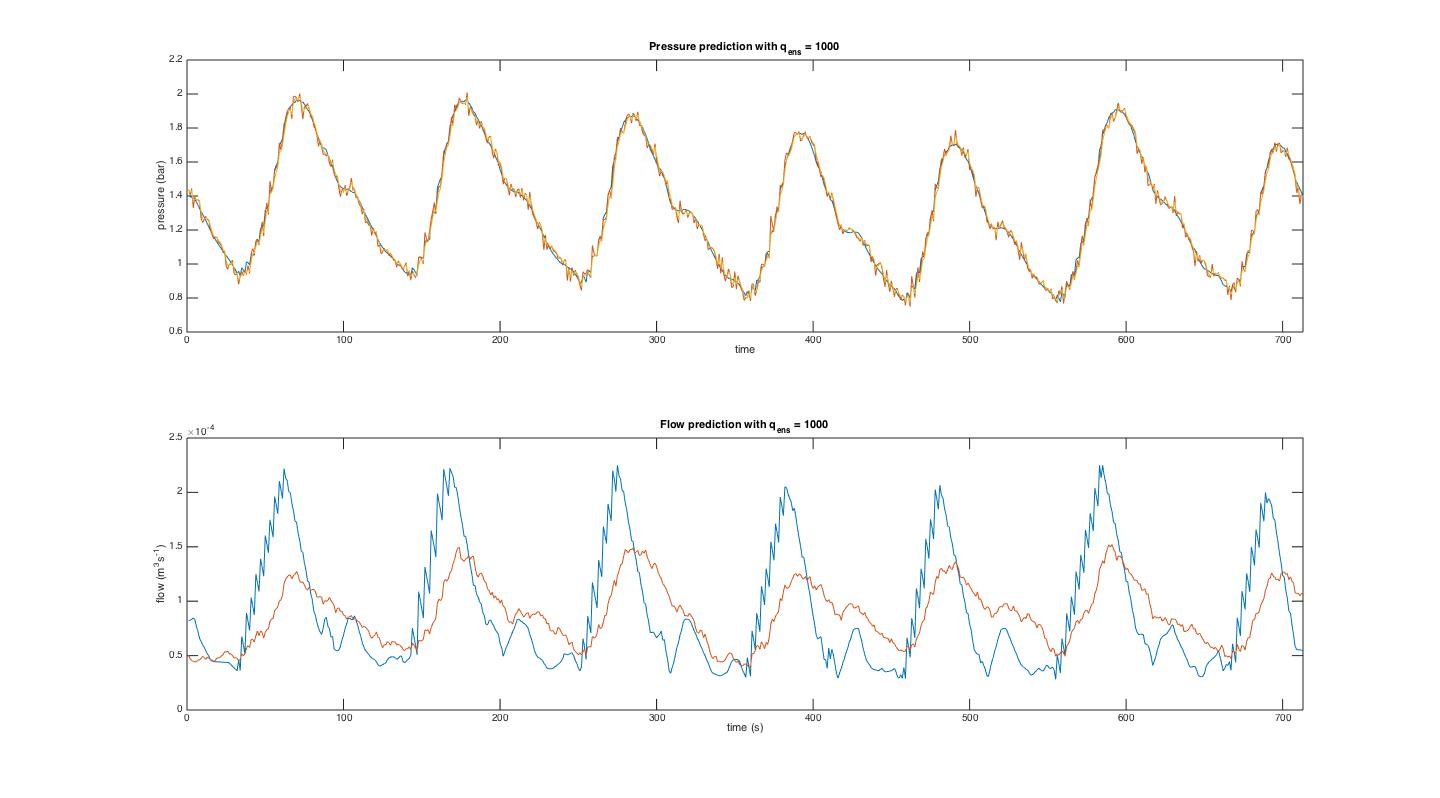
\includegraphics[width=\textwidth]{KFex2}
\end{center}

If $p$ is the real pressure, $y$ its measurement and $x$ its estimation based on $y$, we get a ratio (sum of $(p-y)^2$)/(sum of $(p-x)^2$) = $1.3005$ and a mean square difference between $q$ and its estimation of $2.1087e~10^
{-9}$.

\bigskip

The benefit for direct estimation from measurements of the quantity of interest is quite irrelevant, but the accuracy in indirect estimation is obvious. Further benchmarking in applicable models would be necessary.
\bigskip

Parameter estimation was not successful so far.

\bigskip





\newpage
\chapitre{Unscented Kalman Filters (UKF)}

Ensemble Kalman Filters are interesting for the study of dynamic processes whose models are nonlinear. Intuitively, Extended Kalman Filters (EKF) reduce to linearizing the model and applying standard Kalman Filter. On the other hand, EnKF randomly draw a point cloud around the current state estimation and computes its image through the model in order to estimate the real state. The Unscented Kalman filter (UKF) uses the same kind of method except that the point cloud is replaced with a minimal set of weighted points carefully chosen.


Typically, we consider the state variable $\mathbf x$ is a gaussian random variable whose mean and covariance are denoted $\overline{\mathbf x}$ and $P_{\mathbf x}$. The \emph{sigma-points} set is built to capture the mean and covariance of the state variable as detailed below. This is a consequence of the fact that the forecast and analysis equations of a KF only depend on these two first moments. It is thus sufficient to estimate these statistics.


The UKF has an efficiency comparable to the KF in the linear case and much greater in nonlinear cases. Since we use a restricted set of points for our calculations, it will be less costly than the EnKF. We will be interested in benchmarking these different filters.


As it is written in the PyKalman documentation : "At this point no algorithms have been implemented for inferring parameters". We may be interested in implementing such a tool.



\paragraph{Unscented transformation}~


Predicting state or observation reduces to solving the following problem. Let $\mathbf x$ be a $n-$dimensional gaussian random variable with mean $\mu_{\mathbf x}$ and variance $\Sigma_{\mathbf x}$. If $f$ denotes the function describing our model, let us call $\mu_{\mathbf y}$ and $\Sigma_{\mathbf y}$ respectively the mean and variance of the random variable $\mathbf y=f(\mathbf x)$.


Using the Taylor expansion of $f$ in the neighborhood of $\overline{\mathbf x}$ and assuming the high order terms can be neglected, we get, using convenient notation :

\eq{\begin{array}{l}
\overline{\mathbf y}\simeq f(\overline{\mathbf x})\\
\Sigma_{\mathbf y}\simeq\nabla f\Sigma_{\mathbf x}\nabla f^T
\end{array}}

\noindent The sigma-points set is chosen such that :
\begin{itemize}
\item its mean is $\mu_{\mathbf x}$,
\item its covariance matrix is $\Sigma_{\mathbf x}$.
\end{itemize}

\bigskip

\noindent For $i=1,...,n$ :

\eq{\begin{array}{ll}
X_0=\mu_{\mathbf x}&W_0=\displaystyle\frac\kappa{n+\kappa}\\
X_i=\mu_{ \mathbf x}+\left[\sqrt{(n+\kappa)\Sigma_{\mathbf x}}\right]_i&W_i=\displaystyle\frac1{2(n+\kappa)}\\
X_{n+i}=\mu_{\mathbf x}-\left[\sqrt{(n+\kappa)\Sigma_{\mathbf x}}\right]_i&W_{n+i}=\displaystyle\frac1{2(n+\kappa)}
\end{array}}

\noindent where $\left[M\right]_i$ denotes the $i$th colums of the matrix $M$ and $\sqrt\cdot$ denotes the matrix square root (e.g. using Cholesky decomposition).


We then compute the following :

\eq{\begin{array}{l}
Y_i=f(X_i)~~\text{ for $i=0,...,2n$}\\
\mu_{\mathbf y}\simeq\displaystyle\sum_{i=0}^{2n}W_iY_i\\
\Sigma_{\mathbf y}\simeq\displaystyle\sum_{i=0}^{2n}W_i(Y_i-\mu_{\mathbf y})(Y_i-\mu_{\mathbf y})^T
\end{array}}

According to the authors, when $\mathbf x$ is assumed to be Gaussian, we may take $\kappa$ such that $n+\kappa=3$.

\bigskip

\paragraph{The filter itself}~


We consider the state $x_t$ at each time $t$ is a gaussian random variable $\mathcal N\left(\mu_t,\Sigma_t\right)$ whose statistics are to be estimated. We assume $\mu_0$ and $\Sigma_0$ are known. Then, at each time step, the following are computed :

\begin{enumerate}
\item sigma-points around last state estimate $X$ ,
\item sigma-points propagation through unscented transform : state forecast $\overline X$,
\item recover the forecast mean and covariance $\overline\mu_{\overline X}$ and $\overline\Sigma_{\overline X}$,
\item corresponding measurement forecast $Y$ of mean $\mu_Y$ and covariance $Sigma_Y$,
\item innovation covariance and Kalman gain $\Sigma_{YY}$, $\Sigma_{\overline XY}$ and $K$,
\item state analysis $\mu$.
\end{enumerate}


We performed the following implementation (Octave) of the UKF in a simple case.


\begin{verbatim}
    T = 100;
    dt = 0.2;
    time = (0:T-1)*dt;
    
    sd = 1;
    sd_mes = 0.4;
    n = 1;
    kappa = 2;
    
    x = zeros(1,T);
    for t=2:T
        x(t) = x(t-1) + (1+randn(1)/4)*cos(t*dt)*dt;
    end
    
    y = x + randn(1,T)*sd_mes;
    mu = ones(1,T)*y(1);
    
    Sigma = sd^2;
    W = [kappa/(n+kappa) , 1/(2*(n+kappa)) , 1/(2*(n+kappa))];
    
    for t = 1:T-1
        
            % sigma-points
        X = mu(t) + [0 ; sqrt((n+kappa)*Sigma) ; -sqrt((n+kappa)*Sigma)];
   
            % unscented transform
        Xbar = X + cos(t*dt)*dt;
        
            % mean and covariance predictions
        mubar = W*Xbar;
        Sigmabar = W*((Xbar-mubar).^2);
            
            % measurement predictions
        Ybar = mubar + [0 ; sqrt((n+kappa)*Sigmabar) ; -sqrt((n+kappa)*Sigmabar)];
        yhat = W*Ybar;

            % Kalman gain
        S = W*((Ybar - yhat).^2) + sd_mes^2;
        SigmabarX = W*((Xbar-mubar).*(Ybar-yhat));
        K = SigmabarX/S;
        
        mu(t+1) = mubar + K*(y(t) - yhat);
        Sigma = Sigmabar - K*S*K;
        
    end
\end{verbatim}



\newpage
\chapitre{Comparison}

We first tested the two filters in the same conditions on the previous trivial tracking testcase (complete Octave script available in annex). Since the UKF is deterministic and the EnKF is not, the efficiency of the latter is a random variable we wanted to evaluate precisely. The testcase involving a random parameter, we wanted to perform several runs in order to wipe out this incertainty. That is why we performed 50 runs of tests, each one containing one UKF and 50 EnKF on the exactly same state end measurement sets.


The states on which the benchmark was performed is a noised sinusoid like the following one :

\begin{center}

\resizebox{.6\linewidth}{!}
{

% Title: gl2ps_renderer figure
% Creator: GL2PS 1.4.0, (C) 1999-2017 C. Geuzaine
% For: Octave
% CreationDate: Thu Feb  8 16:51:31 2018
\setlength{\unitlength}{1pt}
\begin{picture}(0,0)
\includegraphics{KFbenchmark-inc}
\end{picture}%
\begin{picture}(576,432)(0,0)
\fontsize{10}{0}
\selectfont\put(74.88,42.519){\makebox(0,0)[t]{\textcolor[rgb]{0.15,0.15,0.15}{{0}}}}
\fontsize{10}{0}
\selectfont\put(187.607,42.519){\makebox(0,0)[t]{\textcolor[rgb]{0.15,0.15,0.15}{{5}}}}
\fontsize{10}{0}
\selectfont\put(300.335,42.519){\makebox(0,0)[t]{\textcolor[rgb]{0.15,0.15,0.15}{{10}}}}
\fontsize{10}{0}
\selectfont\put(413.062,42.519){\makebox(0,0)[t]{\textcolor[rgb]{0.15,0.15,0.15}{{15}}}}
\fontsize{10}{0}
\selectfont\put(69.8755,47.5201){\makebox(0,0)[r]{\textcolor[rgb]{0.15,0.15,0.15}{{3.5}}}}
\fontsize{10}{0}
\selectfont\put(69.8755,117.936){\makebox(0,0)[r]{\textcolor[rgb]{0.15,0.15,0.15}{{4}}}}
\fontsize{10}{0}
\selectfont\put(69.8755,188.352){\makebox(0,0)[r]{\textcolor[rgb]{0.15,0.15,0.15}{{4.5}}}}
\fontsize{10}{0}
\selectfont\put(69.8755,258.768){\makebox(0,0)[r]{\textcolor[rgb]{0.15,0.15,0.15}{{5}}}}
\fontsize{10}{0}
\selectfont\put(69.8755,329.184){\makebox(0,0)[r]{\textcolor[rgb]{0.15,0.15,0.15}{{5.5}}}}
\fontsize{10}{0}
\selectfont\put(69.8755,399.6){\makebox(0,0)[r]{\textcolor[rgb]{0.15,0.15,0.15}{{6}}}}
\end{picture}

}

\end{center}


It is highly relevant to empasize the fact that the EnKF was ran with an ensemble of size 3 ; this comes from our will to compare the efficiency for the same number of point cloud.


The efficiency is defined as the ratio of the $L^2$ norms of the measurement deviation and the estimation deviation. If $x$ denotes the real state array, $y$ the measurements array and $z$ the estimation set, the efficiency is then :

\eq{\eta = \frac{\|x-y\|_2}{\|x-z\|_2}}


We got the following results :

\bigskip

\noindent Ensemble Kalman Filter
\begin{itemize}
\item mean time = 0.17365 s
\item mean efficiency = 2.1928
\end{itemize}
 Unscented Kalman Filter
\begin{itemize} 
\item mean time = 0.010553 s
\item mean efficiency = 1.4729
\end{itemize}

\bigskip

In similar conditions, the UKF is approximately 10 times faster for a slightly worse accuracy than the measurements, while the EnKF is slightly better but much slower and its accuracy is variable.


\bigskip


The second test is about recovering the voltage at the middle-point of a RCR circuit, knowing the rasistances and capacitance and measuring the current input. We denote by $q$ the current input and consider it is given by the previous noised sinusoid.


\begin{center}
\begin{tikzpicture}
\draw (-1.7,0)--(-1.3,0);
\draw (1.3,0)--(1.7,0);
\draw (0,-1)--(0,-1.4);
\draw (-0.7,0)--(0.7,0);
\draw (0,0)--(0,-0.8);

% resistors
\draw (-1.3,0)--(-1.2,0.2)--(-1.1,-0.2)--(-1,0.2)--(-0.9,-0.2)--(-0.8,0.2)--(-0.7,0);
\draw (1.3,0)--(1.2,0.2)--(1.1,-0.2)--(1,0.2)--(0.9,-0.2)--(0.8,0.2)--(0.7,0);

% capacitor
\draw (-0.25,-0.8)--(0.25,-0.8);
\draw (-0.25,-1)--(0.25,-1);

% ground
\draw (-0.25,-1.4)--(0.25,-1.4);
\draw (-0.18,-1.45)--(0.18,-1.45);
\draw (-0.11,-1.5)--(0.11,-1.5);
\draw (-0.06,-1.55)--(0.06,-1.55);

\draw (1.7,0.25)--(1.7,-0.25);
\draw (1.75,0.18)--(1.75,-0.18);
\draw (1.8,0.11)--(1.8,-0.11);
\draw (1.85,0.06)--(1.85,-0.06);

% annotations
\draw (0,0) node [above] {$\pi$};

\draw (-1,0.3) node [above] {$R_1$};
\draw (1,0.3) node [above] {$R_2$};
\draw (0.3,-0.85) node [right] {$C$};

\draw[->] (-2.15,0)--(-1.75,0);
\draw (-2,0) node [above] {$p$};
\draw (-2,0) node [below] {$q$};

\end{tikzpicture}


~


$RCR~network$
\end{center}


Using obvious notations, we want to recover $\pi$ from a measurement of $q_1$. Applying Kirschoff's law :

\eq{
\begin{array}{rl}
q_1=&\displaystyle q_2+q_C\\
=&\displaystyle\frac\pi{R_2}+C\frac{d\pi}{dt}
\end{array}
}

\noindent yielding :

\eq{\pi(t+dt)=\frac{R_2dt}{CR_2+dt}\left(q_1(t+dt)+\frac C{dt}\pi(t)\right)}














\newpage
\chapitre{Annex : tracking comparison}

\begin{verbatim}
clear

T = 100;
dt = 0.2;
time = (0:T-1)*dt;

Nloop = 10;
ukfeff = 0;
ukft = 0;
enkfeff = 0;
enkft = 0;

for L=1:Nloop

    x = 5 + rand*ones(1,T);
    for t=2:T
        x(t) = x(t-1) + (1+randn(1)/4)*cos(t*dt)*dt;    % state is a slightly noised sinusoid
    end

    sd_mes = 0.4;               % measurements are this much accurate
    y = x + randn(1,T)*sd_mes;  % simulated measurements

            % UKF

    mu = ones(1,T)*y(1);        % first state estimate is the measurement
    Sigma = 1;                  % first covariance estimate is arbitrary or fed by extra knowledge

    n = 1;                      % UKF parameter
    kappa = 2;                  %      ''
    
    tic();

    W = [kappa/(n+kappa) , 1/(2*(n+kappa)) , 1/(2*(n+kappa))];  % constant weights

    for t = 1:T-1

        % sigma-points
        X = mu(t) + [0 ; sqrt((n+kappa)*Sigma) ; -sqrt((n+kappa)*Sigma)];

        % unscented transform
        Xf = X + cos(t*dt)*dt;

        % mean and covariance predictions
        muf = W*Xf;
        Sigmabar = W*((Xf-muf).^2);

        % measurement predictions
        Yf = Xf;%mubar + [0 ; sqrt((n+kappa)*Sigmabar) ; -sqrt((n+kappa)*Sigmabar)];
        yhat = W*Yf;

        % innovation covariance
        S = W*((Yf - yhat).^2) + Sigma;
        SigmabarX = W*((Xf-muf).*(Yf-yhat));
        K = SigmabarX/S;

        mu(t+1) = muf + K*(y(t) - yhat);
        %Sigma = Sigmabar - K*S*K;

    end
    
    ukftime = toc();
    ukfefficiency = sqrt(mean((x-y).^2)/mean((x-mu).^2));   % efficiency is the L2 norm ratio of measurement deviation by estimation deviation
    subplot(121)
    plot(time,x,time,y,time,mu)

            % EnKF

    Ntest = 10;
    enkftime = 0;
    enkfefficiency = 0;
    qens = 30;

    mu = ones(1,T)*y(1);        % first state estimate is the measurement
    W = ones(1,qens)/qens;
    
    for I=1:Ntest
        
        tic();

        Xf = randn(qens,1)*sqrt(abs(y(1)))/100 + y(1);
        Xa = Xf;
        Xa_bar = mean(Xa);

        y_kal = zeros(1,qens); % initialisation

        for t=2:T
 
            % propagation
            Xf = Xa + cos(t*dt)*dt;

            % mean predictions
            muf = W*Xf;

            % measurement predictions
            Yf = Xf;
            yhat = W*Yf;
            
            E = randn(qens,1)*sqrt(abs(y(t)))/100;
            y_kal = E + y(t)*ones(qens,1);

            % innovation covariance
            S = var(Yf) + var(E);
            SigmabarX = W*((Xf-muf).*(Yf-yhat));
            K = SigmabarX/S;
            
            for q = 1:qens
                Xa(q) = Xf(q) + K*(y_kal(q) - Yf(q));
            end

            mu(t) = mean(Xa);

        end

            enkftime = enkftime + toc();

            eff = sqrt(mean((x-y).^2)/mean((x-mu).^2));   % efficiency is the L2 norm ratio of measurement deviation by estimation deviation
            enkfefficiency = enkfefficiency + eff;
        
    end

    enkftime = enkftime/Ntest;
    enkfefficiency = enkfefficiency/Ntest;
    subplot(122)
    plot(time,x,time,y,time,mu)
    
    ukfeff = ukfeff + ukfefficiency;
    enkfeff = enkfeff + enkfefficiency;
    ukft = ukft + ukftime;
    enkft = enkft + enkftime;
    
end

ukfeff = ukfeff/Nloop;
enkfeff = enkfeff/Nloop;
ukft = ukft/Nloop;
enkft = enkft/Nloop;

disp(' ')
disp('Ensemble Kalman Filter')
disp(' ')
disp(['    mean time = ',num2str(enkft),' s'])
disp(['    mean efficiency = ',num2str(enkfeff)])
disp(' ')
disp('Unscented Kalman Filter')
disp(' ')
disp(['    mean time = ',num2str(ukft),' s'])
disp(['    mean efficiency = ',num2str(ukfeff)])
disp(' ')


\end{verbatim}



\newpage
\chapitre{Annex : state estimation comparison}

\begin{verbatim}
clear

format long

T = 100;
dt = pi/10;
time = (0:T-1)*dt;

R1 = 1600;
R2 = 13000;
C = 2.5e-5;

p = 5 + rand*ones(1,T);
q=0*p;
for t=2:T
    p(t) = p(t-1) + (1+randn(1)*sqrt(p(1))/10)*cos(t*dt)*dt;    % nodal pressure is a slightly noised sinusoid
end
for t=1:T-1
    q(t+1) = (p(t+1)/R2+C*(p(t+1)-p(t))/dt); % corresponding RCR input current
end
q(1)=q(T);

q = q + randn(1,T)*sqrt(mean(q))/500;

        % UKF

mu = ones(1,T)*q(1)*(C+R2*dt)/(C*R2+dt*R2^2);       % first state estimate
Sigma = 1;                  % first covariance estimate is arbitrary or fed by extra knowledge

n = 1;                      % UKF parameter
kappa = 2;                  %      ''

W = [kappa/(n+kappa) , 1/(2*(n+kappa)) , 1/(2*(n+kappa))];  % constant weights


for t = 1:T-1

    % sigma-points around state
    X = mu(t) + [0 ; sqrt((n+kappa)*Sigma) ; -sqrt((n+kappa)*Sigma)];

    % unscented transform to get predicted state (time update)
    Xbar = R2*dt*(q(t+1)+C*X/dt)/(C*R2+dt);

    % mean and covariance predictions
    mubar = W*Xbar;
    Sigmabar = W*((Xbar-mubar).^2);

    % measurement predictions
    Yf = (1/R2+C/dt)*Xbar - mu(t)*C/dt;
    yhat = W*Yf;

    % innovation covariance
    Cpy = W*((Xbar - mubar).*(Yf - yhat));
    Cyy = W*((Yf - yhat).*(Yf - yhat)) + Sigma;
    K = Cpy/Cyy;

    mu(t+1) = mubar + K*(q(t+1) - yhat);
    %Sigma = Sigmabar - K*Cyy*K';

end

subplot(121)
plot(time,p,time,mu)


    % EnKF

qens = 20;

muen = ones(1,T)*q(1)*(C+R2*dt)/(C*R2+dt*R2^2);       % first state estimate
Sigma = 1;                  % first covariance estimate is arbitrary or fed by extra knowledge

W = ones(1,qens)/qens;

Nloop=1;
meanenerror = 0;
for N = 1:Nloop
    
    Xf = randn(qens,1)*sqrt(abs(q(1))) + q(1);
    Xa = Xf;
    Xabar = W*Xa;
    
    y_kal = zeros(qens,1);
    
for t = 2:T

    % propagation
    Xf = R2*dt*(q(t)+C*Xa/dt)/(C*R2+dt);

    % mean predictions
    muf = W*Xf;
    
    % measurement predictions
    Yf = (1/R2+C/dt)*Xf - muen(t-1)*C/dt;
    yhat = W*Yf;

    % measurement noising
    E = randn(qens,1)*sqrt(abs(q(t)))/100;
    y_kal = E + q(t)*ones(qens,1);

    % innovation covariance
    Cpy = W*((Xf - muf).*(Yf - yhat));
    Cyy = var(Yf) + var(E);
    K = Cpy/Cyy;

    for i = 1:qens
        Xa = Xf + K*(y_kal(i) - Yf(i));
    end
    
    muen(t) = mean(Xa);

end

meanenerror = meanenerror + sqrt(mean((p-muen).^2));
end
meanenerror = meanenerror/Nloop;

subplot(122)
plot(time,p,time,mu)

disp('Mean L2 norm of estimation deviation :')
disp(['    UKF : ',num2str(sqrt(mean((p-mu).^2)))])
disp(['    EnKF : ',num2str(meanenerror)])
\end{verbatim}




\newpage
\chapitre{Bibliography}

J.-F. Gerbeau \emph{A framework for data assimilation in computational hemodynamics  
VIVABRAIN summer school}, PDF (2017)


[ABB17] A. Arnold, C. Battista, D. Bia, Y.Z. German, R.L. Armentano, H. Tran, M.S. Olufsen \emph{Uncertainty quantification in a patient-specific one-dimensional arterial network model : EnKF -based inflow estimator}, Journal of Verification, Validation and Uncertainty Quantification, vol. 2 (2017)


[HSH05] A. Moradkhani, S. Sorooshian, H.V. Gupta, P.R. Houser \emph{Dual state-parameter estimation of hydrological models using ensemble Kalman filter}, Advances in Water Resources 28 (2005) 135–147 (2005)


[JU97] S.J. Julier, J.K. Uhlmann \emph{A New extension of the Kalman Filter to Nonlinear Systems}, Proc. of AeroSence : The 11th Int. Symp. on Aerospace/Defence Sensing, Simulation and Controls (1997)


[KSW16] M. Katzfuss, J.R. Stroud, C.K. Wikle \emph{Understanding the Ensemble Kalman Filter}, The American Statistician vol. 70, n$^\circ$4, 350-357 (2016)


[Lal17] R. Lal \emph{Data assimilation and uncertainty quantification in cardiovascular biomechanics}, thèse (2017)


[TC94] R. Todling, S.C. Cohn \emph{Suboptimal schemes for atmospheric data assimilation based on the Kalman filter}, Data Assimilation Office, NASA/Goddard Space Flight Center, Greenbelt, Maryland (1994)


[WM00] E.A. Wan, R. van der Merwe \emph{The Unscented Kalman Filter for Nonlinear Estimation},  Oregon Graduate Institute of Science \& Technology (2000)




\end{document}